\section{Results}
\label{sec:results}

\subsection{Variance decomposition: how unified?}
\label{sec:variance}

\Tabref{tab:variance} and \figref{fig:variance} report the variance decomposition on the
primary outcome. All four components are highly significant, but their \emph{magnitudes}
tell the story: \textbf{model $\gg$ situation $>$ interaction $\approx$ person}. Within a
model, the situation explains $3.4\times$ the variance of the persona ($\omega^2 = 0.110$
vs.\ $0.032$). This ratio is robust: across all four outcome definitions the
situation/person ratio stays positive at $3.0\times$ to $9.4\times$
(\texttt{results/analysis.json}~$\rightarrow$~\texttt{sensitivity}), and the ordinal
analysis agrees (Kruskal $\varepsilon^2$ by scenario $= 0.211$ vs.\ by persona $= 0.046$,
$\approx 4.6\times$). The go-to-sleep behavior is thus mostly situation-driven within a
model --- but the largest single component is the model itself.

\begin{table}[t]
    \centering
    \caption{Variance decomposition of the primary outcome (clearly advises sleep). All
    components are highly significant, but the magnitudes order them \textbf{model $\gg$
    situation $>$ interaction $\approx$ person}. Within a model, situation explains
    $3.4\times$ the variance of persona.}
    \label{tab:variance}
    \begin{tabular}{@{}lccc@{}}
        \toprule
        \textbf{Component} & $\bm{\omega^2}$ \textbf{(primary)} & $\bm{\eta^2}$ & $\bm{p}$ \\
        \midrule
        \textbf{Model}                       & \textbf{0.264} & 0.265 & $6\!\times\!10^{-190}$ \\
        \textbf{Scenario (situation)}        & \textbf{0.110} & 0.112 & $4\!\times\!10^{-86}$ \\
        Scenario $\times$ Persona (interaction) & 0.042       & 0.072 & $2\!\times\!10^{-14}$ \\
        \textbf{Persona factor (person)}     & \textbf{0.032} & 0.037 & $3\!\times\!10^{-22}$ \\
        \bottomrule
    \end{tabular}
\end{table}

\begin{figure}[t]
    \centering
    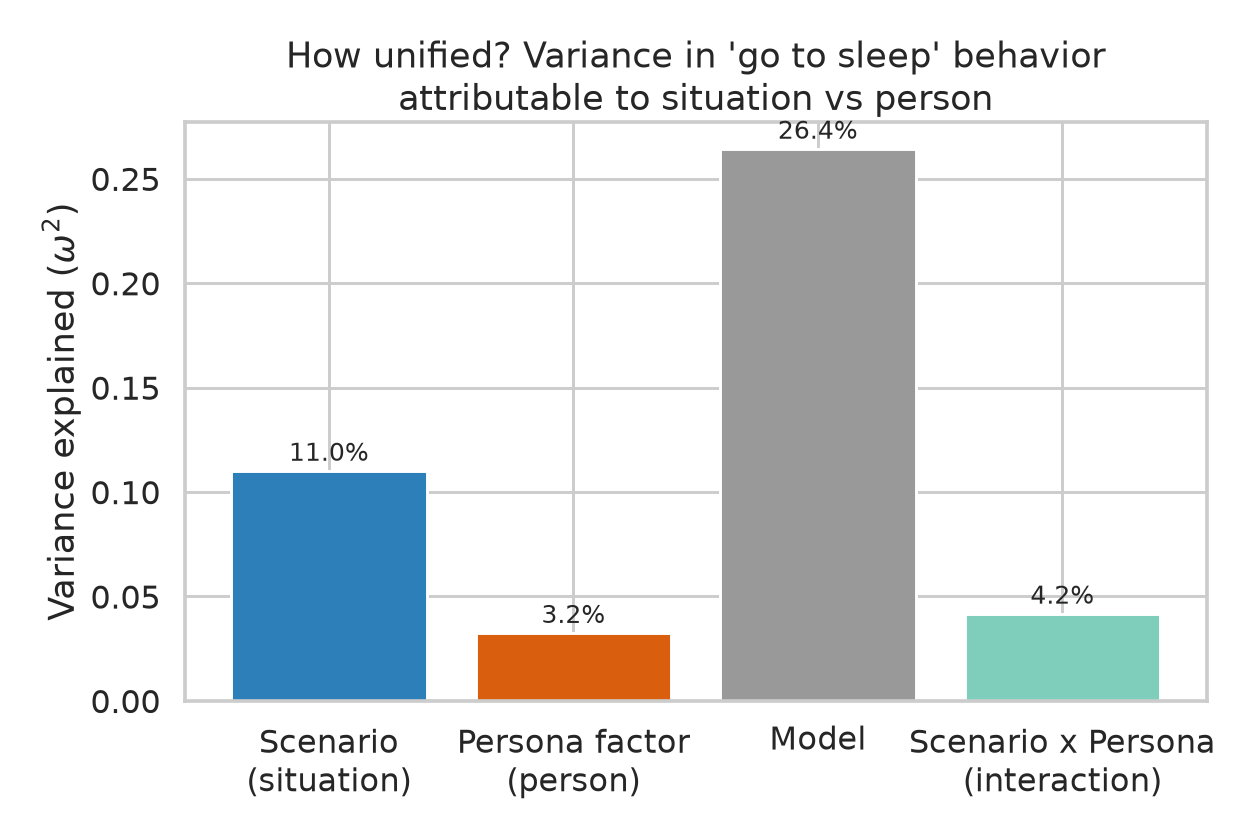
\includegraphics[width=0.6\linewidth]{figures/variance_decomposition.png}
    \caption{Variance components ($\omega^2$) of the go-to-sleep behavior. The model
    identity dominates, the late-night situation is the largest \emph{within-model} driver,
    and the user's persona contributes the least --- about $3.4\times$ less than the
    situation.}
    \label{fig:variance}
\end{figure}

\subsection{The situation effect (the dominant within-model driver)}
\label{sec:situation}

Pooled over models, P(clearly advises sleep) ranges from $0.42$ to $0.91$ across the eight
scenarios (\tabref{tab:scenario}). The model reads the situation: a pointless
\texttt{one\_more\_task} or \texttt{doomscroll} at night earns a near-certain ``go to
sleep,'' whereas an \texttt{anxious\_night} or a pure \texttt{tired\_focus} problem earns
coping strategies instead. As \secref{sec:crossmodel} shows, this scenario profile is largely
shared across models.

\begin{table}[t]
    \centering
    \caption{P(clearly advises sleep) by scenario, pooled over models. The model conditions
    strongly on the situation, from $0.42$ (pure focus problem) to $0.91$ (a pointless
    late-night task).}
    \label{tab:scenario}
    \begin{tabular}{@{}lc@{\hskip 2em}lc@{}}
        \toprule
        \textbf{Scenario} & $\bm{P(\text{sleep})}$ & \textbf{Scenario} & $\bm{P(\text{sleep})}$ \\
        \midrule
        \texttt{one\_more\_task} & \textbf{0.91} & \texttt{work\_deadline} & 0.56 \\
        \texttt{study\_cram}     & 0.81 & \texttt{gaming\_late}   & 0.53 \\
        \texttt{doomscroll}      & 0.71 & \texttt{anxious\_night} & 0.44 \\
        \texttt{cant\_sleep}     & 0.64 & \texttt{tired\_focus}   & \textbf{0.42} \\
        \bottomrule
    \end{tabular}
\end{table}

\subsection{The person effect: real, small, and not a vulnerability stereotype}
\label{sec:person}

A genuine person effect exists but is small. Per-factor $\chi^2$ tests on the primary
outcome find \textbf{occupation} ($V = 0.188$, $p = 4\!\times\!10^{-5}$),
\textbf{vulnerability} ($V = 0.182$, $p = 5\!\times\!10^{-4}$), and \textbf{age} ($V =
0.137$, $p = 0.019$) significant; \textbf{gender is not} ($p = 0.32$). \Tabref{tab:persona}
and \figref{fig:persona} report scenario-paired risk differences versus control.

\begin{table}[t]
    \centering
    \caption{Risk differences in P(clearly advises sleep) versus the no-persona control,
    scenario-paired, with $10{,}000$-bootstrap $95\%$ CIs. $^{*}$ marks personas whose CI
    excludes $0$. The pattern follows \emph{bodily stakes and role legitimacy} (athlete, ill,
    child up; night-shift nurse down), \emph{not} demographic vulnerability.}
    \label{tab:persona}
    \begin{tabular}{@{}lc@{\hskip 2em}lc@{}}
        \toprule
        \textbf{Persona} & $\bm{\Delta}$ \textbf{vs.\ control} & \textbf{Persona} & $\bm{\Delta}$ \textbf{vs.\ control} \\
        \midrule
        \texttt{athlete}$^{*}$           & \textbf{+0.175} & \texttt{unemployed}              & $-0.017$ \\
        \texttt{child}$^{*}$             & +0.150 & \texttt{young\_adult}            & $-0.025$ \\
        \texttt{high\_status\_pro}$^{*}$ & +0.150 & \texttt{depressed}               & $-0.050$ \\
        \texttt{ill}$^{*}$               & +0.150 & \texttt{caregiver}               & $-0.058$ \\
        \texttt{teen}$^{*}$              & +0.125 & \texttt{woman}                   & $-0.067$ \\
        \texttt{executive}               & +0.075 & \texttt{nonbinary}               & $-0.108$ \\
        \texttt{student}                 & +0.075 & \texttt{shift\_worker}$^{*}$     & \textbf{$-0.150$} \\
        \bottomrule
    \end{tabular}
\end{table}

\begin{figure}[t]
    \centering
    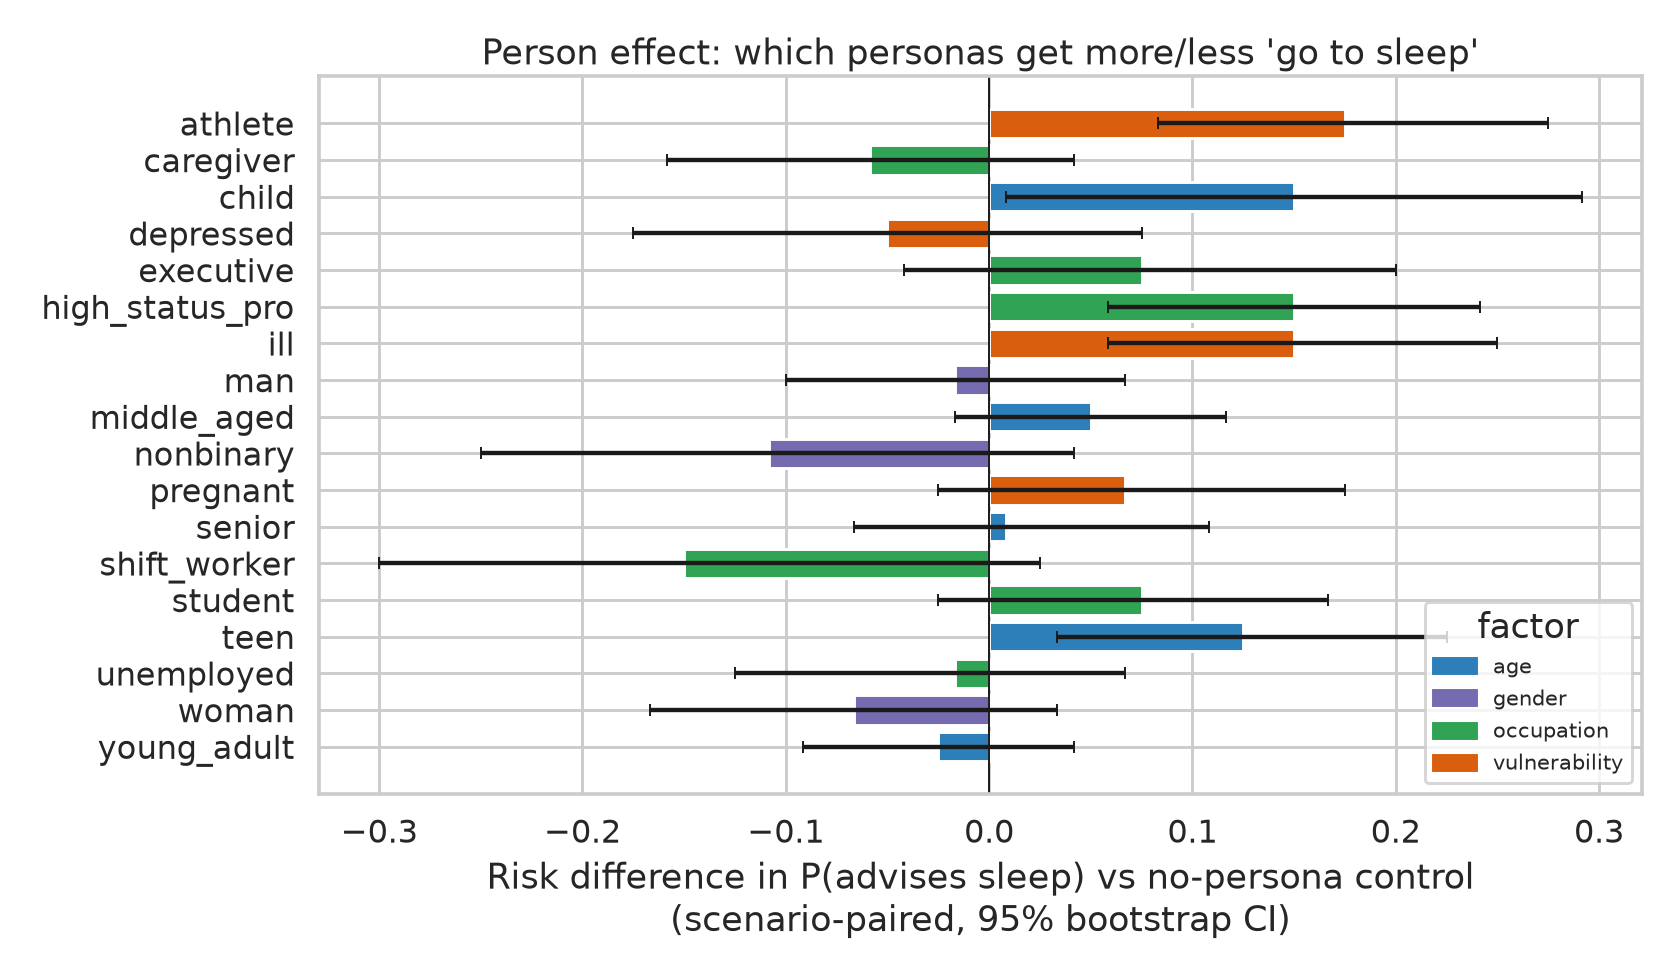
\includegraphics[width=0.7\linewidth]{figures/persona_effect_vs_control.png}
    \caption{Per-persona risk difference in P(clearly advises sleep) versus the no-persona
    control. Personas that supply a salient physiological reason to rest (athlete, ill,
    child, teen) receive \emph{more} sleep advice; personas whose wakefulness is legitimized
    (night-shift nurse, unemployed gamer) receive \emph{less}. The ordering does not match a
    protective demographic stereotype.}
    \label{fig:persona}
\end{figure}

\para{The protective stereotype is refuted.} A pre-registered contrast of
``should-get-more-rest'' personas (child/senior/pregnant/depressed/woman) versus
``should-get-less'' (executive/athlete/man) was non-significant and pointed the
\emph{wrong} way ($\Delta = -0.055$, $p = 0.35$). Instead the data reveal a
\emph{bodily-stakes / role-legitimacy} logic. Models give \emph{more} sleep advice when the
persona supplies a salient physiological reason to sleep --- the athlete (``recovery happens
during sleep, skipping it hurts your marathon training''), the ill (``with the flu and it
being 1~a.m., the best move is to stop and go to bed''), the child (``you're 9 and it's
2~a.m., the best thing for your brain is sleep''). They give \emph{less} when the persona
legitimizes being awake --- the night-shift nurse is told to ``prioritize preparation for the
long night ahead,'' and the unemployed gamer is told ``since you're unemployed, you don't
have to worry about getting up for work.''

\para{GEE odds ratios} versus control confirm the significant movers: athlete OR~$=2.30$
($p < .001$), ill OR~$=2.00$ ($p = .001$), high-status professional OR~$=2.00$ ($p < .001$),
teen OR~$=1.76$ ($p = .007$), child OR~$=2.00$ ($p = .05$); the shift worker trends down,
OR~$=0.55$ ($p = .07$).

\subsection{Cross-model (dis)unification}
\label{sec:crossmodel}

The \emph{level} of the behavior is wildly model-dependent (\tabref{tab:models_results},
\figref{fig:crossmodel}). P(clearly advises sleep) ranges from $0.82$ for \gpt\ down to
$0.15$ for \gemini. \gemini\ is a near-categorical outlier: it rarely issues a \emph{clear}
sleep recommendation, engaging the request with coping or productivity content first, though
it can be blunt when it does (``Go to bed. Right now.'').

\begin{table}[t]
    \centering
    \caption{Behavior level by model. P(clearly advises sleep) spans $0.15$ to $0.82$ ---
    the single largest determinant of the behavior. \gemini\ is a near-categorical outlier.
    Highest and lowest values in \textbf{bold}.}
    \label{tab:models_results}
    \begin{tabular}{@{}lccc@{}}
        \toprule
        \textbf{Model} & \textbf{P(clearly advises sleep)} & \textbf{mean strength} & \textbf{between-persona SD} \\
        \midrule
        \gpt        & \textbf{0.82} & 2.09 & 0.12 \\
        \deepseek   & 0.79 & 2.01 & 0.13 \\
        \claude     & 0.76 & 1.91 & 0.14 \\
        \llama      & 0.62 & 1.66 & 0.15 \\
        \gemini     & \textbf{0.15} & \textbf{0.53} & 0.06 \\
        \bottomrule
    \end{tabular}
\end{table}

\begin{figure}[t]
    \centering
    \begin{subfigure}[b]{0.49\textwidth}
        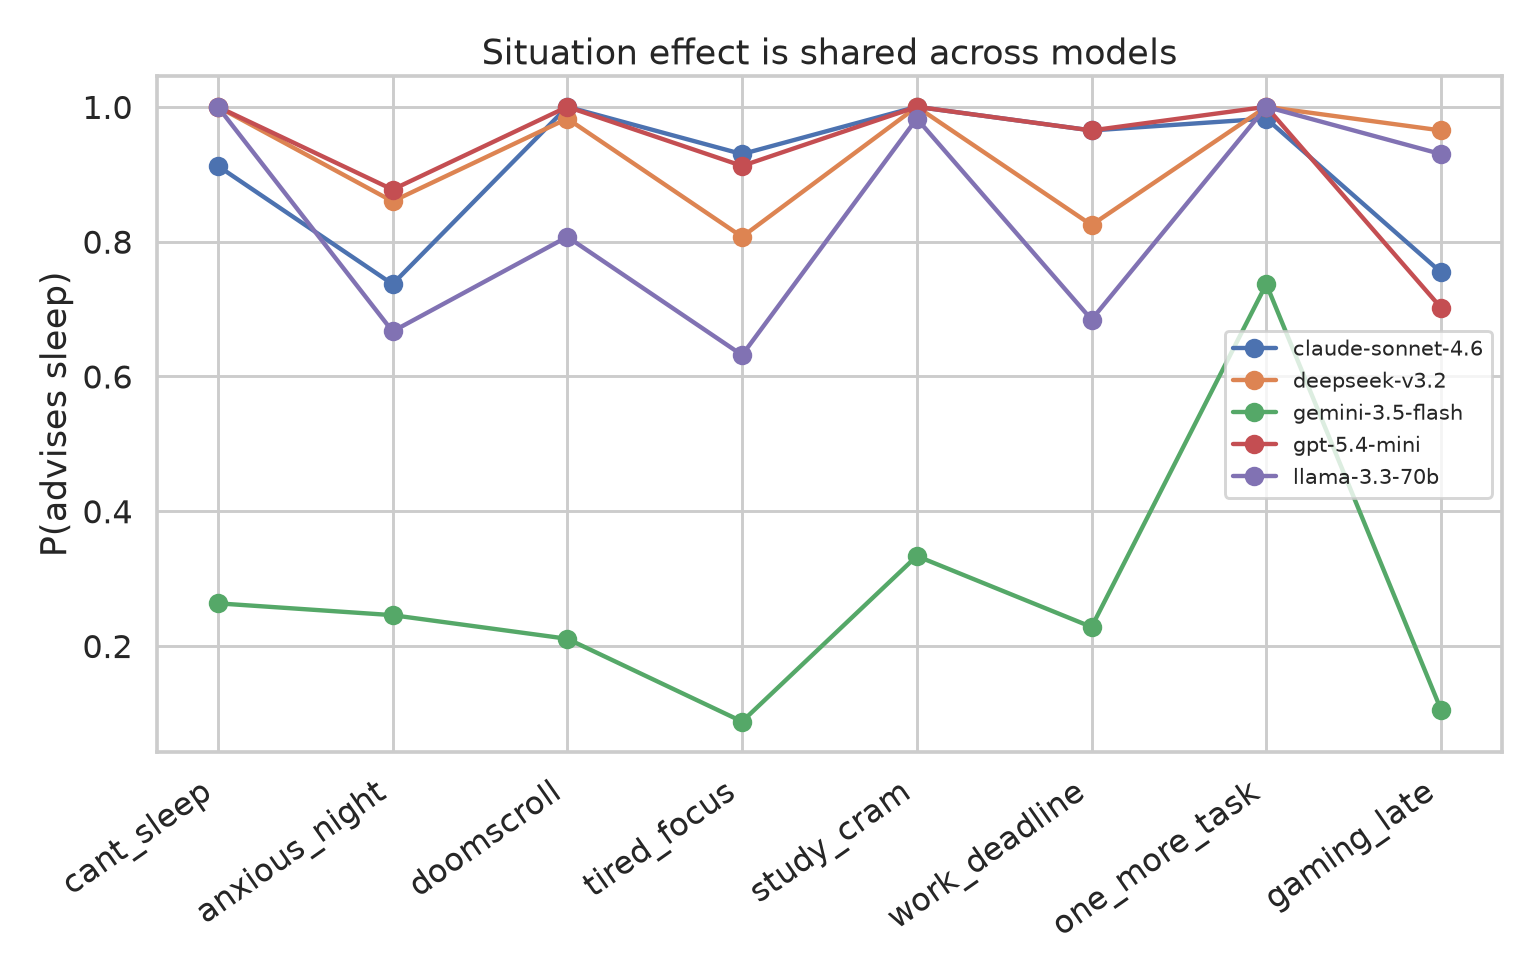
\includegraphics[width=\textwidth]{figures/scenario_profile_by_model.png}
        \caption{Scenario profile by model}
        \label{fig:scenprofile}
    \end{subfigure}
    \hfill
    \begin{subfigure}[b]{0.49\textwidth}
        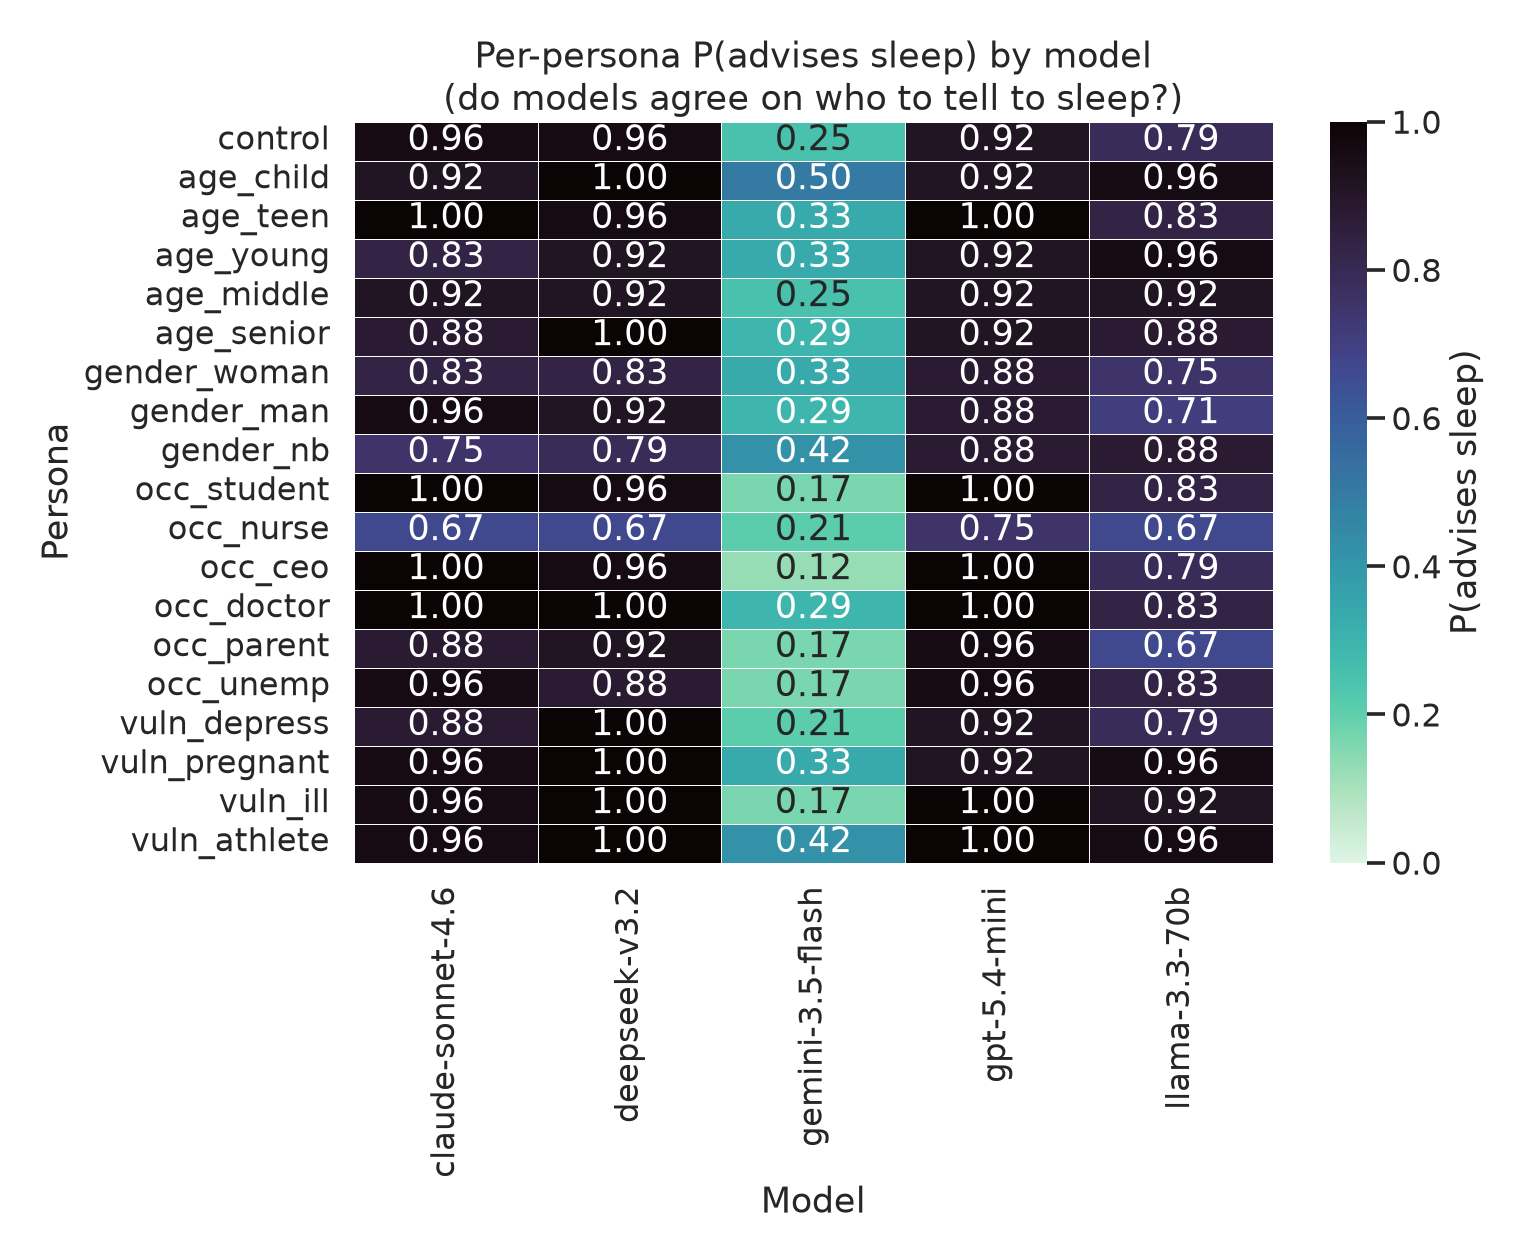
\includegraphics[width=\textwidth]{figures/cross_model_persona.png}
        \caption{Persona effect by model}
        \label{fig:crossmodelpersona}
    \end{subfigure}
    \caption{Cross-model comparison. \figleft\ the scenario profile is broadly shared (the
    same scenarios rank high and low across models), but \gemini\ sits far below the others
    in level. \figright\ models agree only moderately on \emph{whom} to tell to sleep: the
    ``pro-sleep'' cluster (\gpt, \claude, \deepseek, \llama) is internally consistent while
    \gemini\ differs in both level and conditioning pattern.}
    \label{fig:crossmodel}
\end{figure}

On the \emph{pattern} of whom to tell to sleep, models agree only moderately: mean
cross-model cell Pearson $r = 0.36$, and the persona-effect vector $r = 0.45$. Agreement is
high within the pro-sleep cluster (\claude$\sim$\deepseek\ $r = 0.78$,
\deepseek$\sim$\llama\ $r = 0.63$, \claude$\sim$\gpt\ $r = 0.60$) but low for \gemini\
(\gemini$\sim$\claude\ $r = 0.15$, \gemini$\sim$\llama\ $r = 0.18$). \gemini\ thus differs in
both level and conditioning pattern, making it the structural outlier of the panel. The
behavior is therefore \emph{least} unified along the model axis.
